\documentclass[11pt]{article}
\usepackage[T1]{fontenc}
\usepackage{lmodern}
\usepackage[margin=1in]{geometry}
\usepackage{amsmath,amssymb,amsthm}
\usepackage{microtype}
\usepackage{tikz}
\usepackage[hidelinks,hypertexnames=false]{hyperref}
\hypersetup{pdftitle={A two-replica proof of the Krenn--Gu conjecture},pdfauthor={}}
\newtheorem{theorem}{Theorem}[section]
\newtheorem{lemma}[theorem]{Lemma}
\newtheorem{corollary}[theorem]{Corollary}
\theoremstyle{definition}
\newtheorem{definition}[theorem]{Definition}
\theoremstyle{plain}
\numberwithin{equation}{section}
\setlength{\parskip}{0.25em}
\title{A two-replica proof of the Krenn--Gu conjecture}
\author{}
\date{September 26, 2026}
\begin{document}
\maketitle
\begin{abstract}
In the graph model of photonic state preparation, the amplitude of a vertex
colouring is a sum of products of complex edge weights over perfect matchings.
The Krenn--Gu conjecture asks whether these weights can cancel every mixed
colouring while retaining at least three monochromatic colourings on more
than four vertices. We prove that they cannot. The main difficulty is that
the existence of a mixed matching alone does not prevent its amplitude from
cancelling. Our argument forces a stronger structure: after parallel edges
with the same endpoint colours are aggregated, every edge is monochromatic
and every active colour forms a perfect matching. A vertex colouring then
has at most one contributing matching, so a known combinatorial obstruction
finishes the proof. The structural argument uses two identical formal copies
of the matching polynomial. Their symmetries impose polynomial identities
that force each supported edge to contribute the entire amplitude of its
colour. Complex weights, parallel edges, and distinct colours at the two
ends of an edge are all allowed. A Lean formalization verifies the normalized
equation-system statement at every even order at least six and every palette
size at least three.
\end{abstract}

\section{Introduction}\label{sec:introduction}

Perfect matchings provide a bridge between graph theory and the preparation
of entangled states with photon-pair sources. Vertices represent output paths,
edges represent pair contributions, and endpoint colours specify the modes.
Selecting one photon at each output corresponds to selecting a perfect
matching. Contributions that induce the same output modes add as complex
amplitudes; they can therefore interfere destructively. The resulting
existence question was formulated by Krenn, Gu and
Solt\'esz~\cite[Question~1]{kgs}; see also the matching examples
in~\cite[Section~2]{logic}.

For a GHZ target, the desired colourings assign the same colour to every
vertex. All other colourings must have amplitude zero. Graph theory can
force an unwanted matching to exist, but complex weights might cancel its
contribution against other matchings. The proof must therefore explain why
such cancellation cannot satisfy all the target equations simultaneously.
We do this by deriving a structural restriction on the weighted graph itself.

\subsection{Matching amplitudes and the conjecture}\label{sec:graphmodel}

Let \(G=(V,E)\) be a finite loopless multigraph. Each edge \(e=uv\) has
weight \(w(e)\in\mathbb C\) and two endpoint colours \(\chi_u(e),\chi_v(e)\).
We write \([d]=\{1,\ldots,d\}\) for the target palette and
\(\mathcal M(G)\) for the set of perfect matchings of \(G\).
For \(M\in\mathcal M(G)\), let \(e_M(v)\) be its unique edge at \(v\).
The matching induces the vertex colouring
\(v\mapsto\chi_v(e_M(v))\). For a vertex colouring \(\kappa:V\to[d]\), define
\[
 W(\kappa)=
 \sum_{\substack{M\in\mathcal M(G)\\
       \chi_v(e_M(v))=\kappa(v)\ \text{for every }v}}
       \prod_{e\in M}w(e).
\]
An empty sum is zero. We write \(i^V\) for the colouring that is constantly
\(i\). A colouring that is not constant is called mixed. For a matrix \(B\)
and a vertex set \(S\), \(B[S]\) denotes its principal submatrix on \(S\).

\begin{definition}[Generalized GHZ condition]\label{def:ghz}
The weighted half-edge-coloured graph satisfies the generalized GHZ condition
on \([d]\) if \(W(i^V)=\tau_i\ne0\) for every \(i\in[d]\), and
\(W(\kappa)=0\) for every mixed vertex colouring \(\kappa:V\to[d]\).
\end{definition}

The usual normalized condition requires \(\tau_i=1\). Our definitions follow
Chandran, Gajjala and Illickan~\cite[Sections~1.1 and~1.4]{cgi}; the
generalized condition permits unequal nonzero amplitudes.

\begin{theorem}[Krenn--Gu conjecture]\label{thm:graphmain}
If \(|V|>4\) is even, there is no complex weighted half-edge-coloured
multigraph satisfying the generalized GHZ condition on a palette of size
\(d\ge3\).
\end{theorem}

The theorem concerns this matching model with arbitrary complex weights.
There is no restriction on edge density or on the number of parallel edges.
It suffices to retain three active colours: removing edges with other
endpoint colours leaves every amplitude on the retained palette unchanged.

\subsection{Cancellation and the four-vertex boundary}

Consider the left-hand graph in Figure~\ref{fig:examples}. Both of its
perfect matchings induce the mixed colouring \((a,a,b,b)\). Their weights
are \(1\cdot1\) and \(1\cdot(-1)\), so
\[
 W(a,a,b,b)=1\cdot1+1\cdot(-1)=0.
\]
Thus a zero amplitude does not imply the absence of a matching. This small
graph illustrates cancellation only; it does not satisfy the GHZ condition.
The proof has to use the nonzero monochromatic amplitudes together with
the vanishing of \emph{every} mixed amplitude.

\begin{figure}[htbp]
\centering
\begin{minipage}[t]{0.48\textwidth}
\centering
\begin{tikzpicture}[x=1pt,y=1pt,line width=0.8pt]
\path[use as bounding box] (0,0) rectangle (200,116);
\draw[red!70!black] (45,85)--(145,85);
\draw[blue!75!black] (45,25)--(145,25);
\draw[red!70!black] (45,85)--(45,55) (145,85)--(145,55);
\draw[blue!75!black] (45,55)--(45,25) (145,55)--(145,25);
\foreach \x in {45,145} \foreach \y in {25,85}
  \fill (\x,\y) circle (2pt);
\node at (45,101) {\(1:a\)}; \node at (145,101) {\(2:a\)};
\node at (45,9) {\(3:b\)}; \node at (145,9) {\(4:b\)};
\node at (95,95) {\(1\)}; \node at (95,15) {\(1\)};
\node at (31,55) {\(1\)}; \node at (163,55) {\(-1\)};
\end{tikzpicture}

\small (a) Two nonzero matching contributions cancel.
\end{minipage}\hfill
\begin{minipage}[t]{0.48\textwidth}
\centering
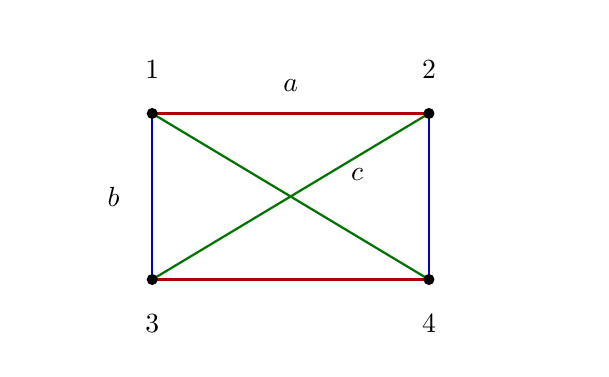
\begin{tikzpicture}[x=1pt,y=1pt,line width=0.8pt]
\path[use as bounding box] (0,0) rectangle (200,116);
\draw[red!70!black] (45,85)--(145,85) (45,25)--(145,25);
\draw[blue!75!black] (45,25)--(45,85) (145,25)--(145,85);
\draw[green!45!black] (45,25)--(145,85) (45,85)--(145,25);
\foreach \x in {45,145} \foreach \y in {25,85}
  \fill (\x,\y) circle (2pt);
\node at (45,101) {\(1\)}; \node at (145,101) {\(2\)};
\node at (45,9) {\(3\)}; \node at (145,9) {\(4\)};
\node at (95,95) {\(a\)}; \node at (31,55) {\(b\)};
\node at (119,63) {\(c\)};
\end{tikzpicture}

\small (b) The four-vertex GHZ construction.
\end{minipage}
\caption{The obstruction and the exceptional case. In (a), labels beside
edges are weights and labels at vertices give the inherited colours; the
two vertical edges have different colours at their ends. In (b), all weights
are one. Horizontal, vertical, and diagonal edges have colours \(a,b,c\),
respectively. The diagonal crossing is not a vertex.}
\label{fig:examples}
\end{figure}

The restriction to more than four vertices is necessary. In
Figure~\ref{fig:examples}(b), the three perfect matchings of \(K_4\) are
\[
 \{12,34\},\qquad \{13,24\},\qquad \{14,23\}.
\]
Colour these matchings \(a,b,c\), respectively, and give every edge weight
one. The only induced colourings are \(a^V,b^V,c^V\), each with amplitude
one. Our structural argument will recover precisely the feature visible in
this example: each colour forms a perfect matching. The final graph
obstruction then distinguishes four vertices from larger orders.

\subsection{Related work}

Chandran and Gajjala use edge pruning and a sparse representative subgraph
to bound the dimension of simple GHZ experiment graphs~\cite{cg}.
Chandran, Gajjala and Illickan prove the conjecture for graphs of vertex
connectivity at most two and for graphs of maximum degree at most three.
Their reduction also implies that a counterexample with the fewest vertices
must be four-connected~\cite[Theorems~9--11]{cgi}. These results concern the
same weighted model.

A separate result, attributed to Bogdanov in~\cite[Theorem~7]{cgi}, states
that three monochromatic perfect matchings of distinct colours on more than
four vertices force a mixed perfect matching. This is an existence statement.
In the complex weighted setting, different matchings may cancel, so it does
not by itself settle the conjecture. Our structural argument removes this
possibility before invoking the combinatorial obstruction.

\subsection{Proof overview: forcing one edge per colour}\label{sec:overview}

We first remove an ambiguity caused by parallel edges. For fixed vertices
\(u,v\) and fixed endpoint colours \(i,j\), replace all corresponding
parallel edges by one edge whose weight is their sum. Delete that edge if
the sum is zero. A perfect matching uses at most one edge between \(u\) and
\(v\), so distributivity shows that this operation preserves every
\(W(\kappa)\). All support and uniqueness statements below refer to this
\emph{aggregate graph}.

The argument has two structural steps and a short combinatorial conclusion.
We describe the conclusion first far enough to make the role of each
structural step explicit.

\paragraph{Step 1: every remaining edge has equal endpoint colours.}
Lemma~\ref{lem:diagonal} proves that every aggregate weight with distinct
endpoint colours is zero. After this reduction, fix an active colour and
write \(B_{pq}\) for its weight on the edge \(pq\). A supported edge means
one with \(B_{pq}\ne0\). Let \(\beta\ne0\) be the amplitude of the
monochromatic colouring in this colour.

\paragraph{Step 2: each supported edge contributes the entire amplitude.}
For an edge \(pq\), define its matching subtotal
\[
 C_{pq}=\sum_{\substack{M\text{ a perfect matching of this colour}\\pq\in M}}
              \prod_{e\in M}w(e).
\]
The central identity, proved in Theorem~\ref{thm:endpoint}, is
\[
 \boxed{C_{pq}=\beta\quad\text{whenever }B_{pq}\ne0.}
\]
Its consequence is immediate. Every perfect matching uses exactly one edge
at a fixed vertex \(p\). If \(\deg_B(p)\) counts the supported edges of
this colour at \(p\), then
\[
 \beta=\sum_{q:\,B_{pq}\ne0}C_{pq}=\deg_B(p)\,\beta.
\]
Since \(\beta\ne0\), we obtain \(\deg_B(p)=1\). This applies to every
vertex and every active colour: each colour graph is a perfect matching.
In particular, the conclusion uses complex amplitudes directly and requires
no positivity argument.

\paragraph{Step 3: a mixed matching can no longer cancel.}
Given a vertex colouring \(\kappa\), its colour at each vertex specifies
the only possible incident edge in a contributing matching. Consequently
there is at most one such matching. If it exists, its weight is a product
of nonzero edge weights and hence is nonzero. But three monochromatic
perfect matchings of distinct colours on more than four vertices force a
mixed perfect matching~\cite[Theorem~7]{cgi}. Its nonzero amplitude
contradicts the GHZ condition. We include the graph argument in
Section~\ref{sec:graph}.

\paragraph{Where the algebra enters.}
The difficult work is to establish Steps 1 and 2. A matching subtotal can be
written as
\[
 C_{pq}=B_{pq}\,\mathrm{haf}\bigl(B[V\setminus\{p,q\}]\bigr),
\]
where the hafnian is the sum of products over perfect matchings on the
remaining vertices. Thus Step 2 is an identity relating a full matching
sum to a sum with two vertices removed. The remaining graph is not assumed
to satisfy any GHZ condition; the identity must follow from the equations
on the original graph.

We obtain such identities by taking two identical formal copies of the
matching polynomial. Mixing the copies preserves their pairing data, while
certain alternating expressions change sign. This yields vanishing
identities that are not visible in a single matching sum. A second use of
the symmetry restricts an auxiliary matrix to a small family of polynomial
forms. The original matching equations then impose differential equations
on their coefficients. A polynomial of positive degree cannot satisfy
\(p'+\delta p=k\) when \(\delta\ne0\) and \(k\) is constant: its
highest-degree term would have nothing to cancel. This finite-degree
argument gives the supported-edge identity.

Section~\ref{sec:model} develops the pairing language from a four-factor
example. Sections~\ref{sec:higher} and~\ref{sec:diagonal} establish Step 1;
Section~\ref{sec:endpoint} proves the identity in Step 2. The final two
steps above are completed in Sections~\ref{sec:matching} and~\ref{sec:graph}.
Section~\ref{sec:scope} states the precise formalization scope.

\section{Algebraic formulation and formal pairings}\label{sec:model}

\subsection{Encoding a matching sum}

Our first algebraic operation enforces the matching rule: a vertex may be
used only once. Associate a variable \(x_{v,i}\) with colour \(i\) at
vertex \(v\), and set every product \(x_{v,i}x_{v,j}\) to zero. Thus a
product of edges sharing a vertex vanishes, regardless of their colours.
Products of vertex-disjoint edges survive.

Write \(n=|V|\) and fix an ordering of \(V\).
Let \(A_{uv}(i,j)\) be the sum of the weights of edges whose endpoint colours
are \(i\) at \(u\) and \(j\) at \(v\), as in the aggregation in
Section~\ref{sec:overview}. The algebra and its edge polynomial are
\[
 \begin{aligned}
 \mathcal A_V&=\mathbb C[x_{v,i}:v\in V,\ i\in\{a,b,c\}]
       \big/\bigl(x_{v,i}x_{v,j}:v\in V,\ i,j\in\{a,b,c\}\bigr),\\
 A&=\sum_{u<v}\sum_{i,j\in\{a,b,c\}}A_{uv}(i,j)x_{u,i}x_{v,j}.
 \end{aligned}
\]
Every surviving term in its divided top power chooses each vertex exactly once.
The division by \((n/2)!\) removes the ordering of the chosen edges. Thus the
coefficient of \(\prod_v x_{v,\kappa(v)}\) is exactly \(W(\kappa)\).
We use \(A^{[j]}=A^j/j!\) for these divided powers. For one colour on four
vertices, the coefficient is the familiar three-term matching sum
\[
 \mathrm{haf}(B)=B_{12}B_{34}+B_{13}B_{24}+B_{14}B_{23}.
\]
In general, \(\mathrm{haf}(B[S])\) denotes the corresponding sum on the
even vertex set \(S\), with value one when \(S\) is empty.

We may therefore express the ternary instance of
Definition~\ref{def:ghz} as follows. Write \(a_v,b_v,c_v\) for the three
coordinates at \(v\), and \(h^S=\prod_{v\in S}h_v\).

\begin{theorem}[Algebraic form of Theorem~\ref{thm:graphmain}]\label{thm:main}
Let \(V\) have even cardinality \(n>4\). In the algebra \(\mathcal A_V\),
let \(A\) be any quadratic involving only distinct vertices, with arbitrary
complex coefficients. Then
\begin{equation}
 A^{[n/2]}=\tau_a a^V+\tau_b b^V+\tau_c c^V,
 \qquad \tau_a\tau_b\tau_c\ne0
 \tag{1}\label{eq:target}
\end{equation}
is impossible.
\end{theorem}

The coefficient interpretation just proved identifies this statement with
the graph theorem after palette restriction. The algebra keeps the original
complex weights, including all aggregate bichromatic weights.

\subsection{Normalizing nonzero target amplitudes}\label{sec:normalization}

The written argument works directly with the nonzero \(\tau_i\) in
\eqref{eq:target}. To compare it with the formally checked statement, it is
useful to give the normalization explicitly. Fix one vertex \(r\).
Multiply each edge incident on \(r\), with colour \(i\) at that endpoint,
by \(\tau_i^{-1}\). Every perfect matching contains exactly one such edge,
so the new amplitude of a colouring \(\kappa\) is
\[
 W'(\kappa)=\tau_{\kappa(r)}^{-1}W(\kappa).
\]
Every pure amplitude becomes one and every mixed amplitude remains zero.
Conversely, a normalized solution already satisfies the generalized
condition. This proves the equivalence without choosing roots of complex
numbers; compare the scaling lemma in~\cite[Lemma~14]{cgi}.

\subsection{Formal pairings: a four-factor example}\label{sec:pairings}

A second algebraic description lets us exploit symmetry. Assign symmetric
pairing coefficients \(c_{ij}=c_{ji}\) to formal symbols \(z_i,z_j\).
Define the pairing sum, also called a formal Wick moment, by summing over
all pairings of the labelled occurrences. For four factors it is
\[
 \mathcal W(z_1z_2z_3z_4)
 =c_{12}c_{34}+c_{13}c_{24}+c_{14}c_{23}.
\]
This is exactly a matching sum. For any even number of factors the same
rule applies; an odd number has moment zero, and the empty product has
moment one. Repeated symbols still have distinct labelled occurrences.
We extend the rule multilinearly to linear combinations of symbols.

The coefficients \(c_{ij}\) are traditionally called covariances, but here
they are arbitrary complex numbers or polynomial parameters. No probability
distribution, positivity, or invertibility is required. This is the algebraic
pairing formula underlying Isserlis's moment formula~\cite{isserlis}.
In particular, a linear substitution preserving all pairwise covariances
preserves every moment: each summand uses only those covariances.

\subsection{Why take two copies?}\label{sec:twocopies}

Take two copies \(X_i,Y_i\) with identical within-copy covariances and zero
cross-copy covariances. For example, the change of variables
\[
 X'_i=\frac{X_i+Y_i}{\sqrt2},\qquad
 Y'_i=\frac{X_i-Y_i}{\sqrt2}
\]
preserves all pairing data: both new copies have the original covariances,
and their cross covariances are still zero. More generally, any complex
orthogonal matrix acting on the two copy labels has this property.
The graph vertices and edge weights remain fixed.

There is also an expression that detects the determinant of this change of
copy coordinates. Choose distinct colours \(\alpha_i,\beta_i\) at a
vertex and form
\[
 \Delta_i=X_{i,\alpha_i}Y_{i,\beta_i}
             -X_{i,\beta_i}Y_{i,\alpha_i}.
\]
Under a copy transformation \(O\), this expression becomes
\((\det O)\Delta_i\). A reflection therefore changes the sign of a product
of \(\Delta_i\)'s on an odd set of vertices. If the remaining factors in
a moment are fixed by that reflection, invariance of the moment forces it
to vanish. Section~\ref{sec:higher} chooses those factors and the reflection
to obtain identities for the original source rows.

On an even set of vertices the product instead stays unchanged. This gives
the invariant pairing used in Section~\ref{sec:endpoint}. Its polynomial
dependence on auxiliary parameters is essential: degree comparisons turn
the symmetry constraints into exact identities. All parameter variations
take place in these auxiliary expressions, with the original edge weights
held fixed. We never assume that deleting vertices preserves the GHZ
condition.

\section{Whole binary higher responses vanish}\label{sec:higher}

The following lemma combines the reflection and common-factor argument
of~\cite{factors}, the two-colour mixed-coefficient identity of~\cite{mixed},
and the finite-degree pure-response argument of~\cite{pure}. We give the
complete proof, including the terminal response.

\begin{lemma}[Whole binary higher-response vanishing]\label{lem:higher}
Let \(\Omega\) have \(2m+1\ge3\) vertices, let \(R\) be an arbitrary quadratic
on \(\Omega\), and let \(D\) be a vector space of rows \(L\) such that
\begin{equation}
 \Phi(L)=L R^{[m]}=\sum_h f_h(L)h^\Omega.
 \tag{2}\label{eq:root}
\end{equation}
Assume all three linear functions \(f_h\) are nonzero and at least two are
independent. For odd \(p\le2m+1\), define
\[
 H_p(L)=L^p R^{[(2m+1-p)/2]}.
\]
For every \(p\ge3\), the tensor \(H_p(L)\) has zero coefficient on every word
using at most two colours, including the terminal degree \(p=2m+1\).
The same vanishing holds after polarization for products of arbitrary rows
from the same \(D\).
\end{lemma}

\begin{proof}
Give formal variables \(X_{i,h}\) their \(R\) covariances, zero covariances
within a vertex, and give an auxiliary \(g\) covariance \(L_i(h)\) with
\(X_{i,h}\) and zero covariance with itself. A Wick moment with \(p\) copies
of \(g\) and one specified coordinate at each vertex is the corresponding
coefficient of \(H_p(L)\). The \(p!\) assignments of auxiliary occurrences
are precisely those of the raw power \(L^p\); the divided power of \(R\)
counts each remaining matching once.

Take two independent identical replicas \((X,g_1)\), \((Y,g_2)\). Choose
distinct local colours \(\alpha_i,\beta_i\) at each vertex and set
\[
 \Delta_i=X_{i,\alpha_i}Y_{i,\beta_i}
              -X_{i,\beta_i}Y_{i,\alpha_i}.
\]
Over \(\mathbb C(s,t)\), the orthogonal reflection
\[
 \frac{1}{s^2+t^2}
 \begin{pmatrix}s^2-t^2&2st\\2st&t^2-s^2\end{pmatrix}
\]
fixes \(sg_1+tg_2\) and negates each \(\Delta_i\). It preserves the replicated
covariance, so the moment of
\[
 (sg_1+tg_2)^{p+1}\prod_{i\in\Omega}\Delta_i
\]
is zero: there are an odd number of determinants. Extracting \(s^pt\) gives
\begin{equation}
 \sum_{I\subseteq\Omega}(-1)^{|I|}H_p(L)(w_I)\Phi(L)(w'_I)=0,
 \tag{3}\label{eq:reflection}
\end{equation}
where \(w_I\) uses \(\beta\) on \(I\) and \(\alpha\) elsewhere, and \(w'_I\)
is complementary. Equality over \(\mathbb C(s,t)\) gives a polynomial identity,
including isotropic parameter values by extension. No operation on the
original source is being made.

With constant local pair \(a,b\), \eqref{eq:reflection} says
\[
 f_b[a^\Omega]H_p=f_a[b^\Omega]H_p.
\]
Two independent \(f\)'s are coprime in \(\mathbb C[D]\), hence for
\(p=2r+1\) there is a common homogeneous polynomial \(q_r\) of degree
\(2r\) such that \([h^\Omega]H_p=f_hq_r\) for every \(h\); \(q_0=1\).
For a mixed word \(w\) avoiding an active colour \(h\), choose
\(\alpha_i=w_i\), \(\beta_i=h\). The only constant complementary word in
\eqref{eq:reflection} is \(h^\Omega\), giving \(f_h[w]H_p=0\). Polynomial
cancellation proves all binary mixed coefficients zero, even at individual
rows where \(f_h(L)=0\).

Define finite polynomials
\[
 \Psi(L)=\sum_{r=0}^m\frac{H_{2r+1}(L)}{(2r+1)!},
 \qquad
 g(L)=\sum_{r=0}^m\frac{q_r(L)}{(2r+1)!}.
\]
On any binary palette \(a,b\), \(\Psi(L)\) thus equals
\[
 g(L)\bigl(f_a(L)a^\Omega+f_b(L)b^\Omega\bigr).
\]
For two tensors on \(\Omega\), let \(K\) be the product of local alternating
pairings, normalized by \(K(a^\Omega,b^\Omega)=1\). Wick moments with shifted
variables \(X_i+L_i\) show that \(K(\Psi(L),\Psi(M))\) is invariant under
simultaneous \(\mathrm{SO}(2)\) rotation of the two mean rows: the replica
covariance and each determinant are unchanged. Choose independent
\(f_a,f_b\). This pairing is
\[
 \bigl(f_a(L)f_b(M)-f_b(L)f_a(M)\bigr)g(L)g(M).
\]
The determinant factor is a nonzero polynomial and is rotation invariant.
Cancel it in \(\mathbb C[D\times D]\), then rotate by \(45\) degrees and set
\(M=0\). Since \(g\) is even and \(g(0)=1\),
\[
 g(L/\sqrt2)^2=g(L).
\]
If \(g\) had positive degree, the degrees of the two sides would differ.
Thus \(g=1\), and all \(q_r\) with \(r\ge1\) vanish. Together with
\eqref{eq:reflection}, this proves whole binary vanishing through the
terminal degree \(2m+1\). Polarization gives the same statement for products
of arbitrary rows from this same \(D\).
\end{proof}

For a source \eqref{eq:target}, delete any root \(p\). Its three actual
incident rows have responses \(\tau_hh^{V\setminus\{p\}}\), so their span
satisfies \eqref{eq:root} with three independent \(f_h\). Thus
Lemma~\ref{lem:higher} applies at every original root, before diagonalization.

\section{Even omission identities and diagonal reduction}\label{sec:diagonal}

The even-omission argument originates in~\cite{omission}. Its role is to
convert the rooted identities into off-diagonal matrix identities.

\begin{lemma}[Even omission]\label{lem:omission}
In the setting of \eqref{eq:root}, omit a vertex \(q\), put
\(S=\Omega\setminus\{q\}\), and write
\[
 \begin{aligned}
 R&=Q+\sum_h h_q V_h,& L&=U+\sum_h d_hh_q,\\
 E(U)&=\sum_{r=0}^m\frac{U^{2r}}{(2r)!}Q^{[m-r]},&F&=E(0).
 \end{aligned}
\]
For any \(L_1,L_2\in D\) and any active colour \(k\),
\[
 [k^S]\,U(L_1)U(L_2)Q^{[m-1]}=0.
\]
This includes \(m=1\).
\end{lemma}

\begin{proof}
The full coefficient of \(q=h\) in \(\Psi(L)\) is
\[
 d_h E(U)+E_{V_h}(U),
\]
where subscripts mean directional derivatives in the mean, with \(Q\)
fixed. By Lemma~\ref{lem:higher}, its projection onto any palette \(h,k\)
on \(S\) is \(f_h(L)h^S\). All the following pairings use this binary
projection implicitly.

Because \(|S|\) is even, \(K\) is symmetric and \(K(Z,h^S)=[k^S]Z\).
The same two-replica rotation gives
\begin{equation}
 \begin{aligned}
 K(E(U),E(U))&=K(F,E(\sqrt2U)),\\
 K(E(U),E_V(U))&=\frac{1}{\sqrt2}K(F,E_V(\sqrt2U)).
 \end{aligned}
 \tag{4}\label{eq:covariance}
\end{equation}
The second identity follows by differentiating the rotation identity at
means \(U,U+tV\): the second rotated mean is zero at \(t=0\) and
\(E'(0)=0\). Substitute
\[
 E_{V_h}(U)=f_hh^S-d_hE(U)
\]
and the corresponding identity for \(\sqrt2L\) into the second equation
of \eqref{eq:covariance}. The first cancels the \(d_h\) terms, leaving
\[
 f_h(L)[k^S]\bigl(E(U)-F\bigr)=0.
\]
Cancel the nonzero polynomial \(f_h\). Separating homogeneous degrees and
polarizing yields
\begin{equation}
 [k^S]\,U(L_1)U(L_2)Q^{[m-1]}=0.
 \tag{5}\label{eq:omission}
\end{equation}
\end{proof}

We next apply this identity to the actual hafnian cofactors. This is the
diagonal reduction proved in~\cite{diagonal}.

\begin{lemma}[Global diagonal reduction]\label{lem:diagonal}
Every endpoint-colour edge block of a source \eqref{eq:target} is diagonal
in the given target coordinates.
\end{lemma}

\begin{proof}
For a fixed colour \(h\), define
\[
 \begin{aligned}
 M_h[p,r]&=A_{pr}(h,h) &&(p\ne r),& M_h[p,p]&=0,\\
 C_h[r,q]&=\operatorname{haf}\bigl(M_h[V\setminus\{r,q\}]\bigr)
                  &&(r\ne q),& C_h[q,q]&=0,\\
 B_{ih}[p,r]&=A_{pr}(i,h) &&(p\ne r),& B_{ih}[p,p]&=0.
 \end{aligned}
\]
Expansion of the original one-defect word at \(p\) gives
\[
 (B_{ih}C_h)[p,p]=\delta_{i,h}\tau_h.
\]
For \(p\ne q\), expand each \(C_h[r,q]\) at its retained vertex \(p\):
\begin{equation}
 \begin{aligned}
 (B_{ih}C_h)[p,q]
 &=\sum_{\substack{r,s\in V\setminus\{p,q\}\\r\ne s}}
       A_{pr}(i,h)A_{ps}(h,h)\,
       \operatorname{haf}\bigl(M_h[V\setminus\{p,q,r,s\}]\bigr)\\
 &=0.
 \end{aligned}
 \tag{6}\label{eq:cofactor}
\end{equation}
The last expression is exactly \eqref{eq:omission} for two rows of the
original \(p\) family after omitting \(q\). Both sums are ordered; there
is no factor \(1/2\). Consequently
\[
 B_{ih}C_h=\delta_{i,h}\tau_h I.
\]
Taking \(i=h\) proves \(C_h\) invertible. Taking \(i\ne h\) then proves
\(B_{ih}=0\). Every original edge block is therefore diagonal. This uses
neither cofactor nonvanishing assumptions nor a change of basis.
\end{proof}

\section{The supported-edge identity}\label{sec:endpoint}

The construction in this section is the finite two-replica endpoint argument
of~\cite{endpoint}. Its inputs are the original root identities obtained
above; the auxiliary parameters do not change the edge weights.

Fix two colours \(B,H\) after diagonal reduction and roots \(p\ne q\).
Put \(U=V\setminus\{p,q\}\), \(N=|U|\) (even), and let \(Q\) be the literal
binary quadratic on \(U\). Write
\[
 \begin{aligned}
 d&=B_{pq},&e&=H_{pq},&\beta&=\operatorname{haf}(B),\\
 \eta&=\operatorname{haf}(H),&\alpha&=\operatorname{haf}(B[U]),\\
 x&=\sum_{i\in U}B_{pi}b_i,& y&=\sum_{i\in U}B_{qi}b_i,\\
 u&=\sum_{i\in U}H_{pi}h_i,& v&=\sum_{i\in U}H_{qi}h_i,\\
 E(L)&=\sum_{j=0}^{N/2}\frac{L^{2j}}{(2j)!}Q^{[N/2-j]},&F&=E(0).
 \end{aligned}
\]

\begin{theorem}[Supported endpoint identity]\label{thm:endpoint}
For every supported edge \(B_{pq}\ne0\),
\[
 \beta=B_{pq}\operatorname{haf}\bigl(B[V\setminus\{p,q\}]\bigr).
\]
\end{theorem}

Derivatives of \(E\) always keep \(Q\) fixed. Lemma~\ref{lem:higher}, applied
to the original \(p\) and \(q\) row planes and expanded at the other root,
gives the exact polynomial identities
\begin{equation}
 \begin{aligned}
 E_y(sx+tu)+dsE(sx+tu)&=s\beta b^U,\\
 E_v(sx+tu)+etE(sx+tu)&=t\eta h^U,\\
 E_x(ay+bv)+daE(ay+bv)&=a\beta b^U,\\
 E_u(ay+bv)+ebE(ay+bv)&=b\eta h^U.
 \end{aligned}
 \tag{7}\label{eq:boundary}
\end{equation}
These include the highest coefficient, which uses the terminal original odd
response of degree \(N+1\). They are identities in mean parameters on the
unchanged source. Differentiating those parameters is legitimate and gives
\begin{equation}
 \begin{aligned}
 E_u(ay)&=0,&E_v(sx)&=0,\\
 E_{yu}(sx)&=-dsE_u(sx),\\
 E_{uv}(sx)+eE(sx)&=\eta h^U,\\
 E_{xy}(0)+dF&=\beta b^U.
 \end{aligned}
 \tag{8}\label{eq:specializations}
\end{equation}

On tensors on \(U\), use the symmetric binary alternating pairing \(K\),
normalized by \(K(b^U,h^U)=1\). The polynomial
\(K(E(L_1),E(L_2))\) is invariant under the full \(\mathrm O(2)\) action
on the two means. The Wick proof is as in Section~\ref{sec:higher}; a
determinant \(-1\) transformation contributes \((-1)^N=1\).

Introduce independent columns \(P,Q_c,R_c,S_c\in\mathbb C^2\) and means
\(L_i=P_i x+(Q_c)_iy+(R_c)_iu+(S_c)_iv\). Set
\[
 \begin{aligned}
 G&=K(E(L_1),E(L_2)),& f&=G\big|_{R_c=S_c=0},\\
 M_{ij}&=\left.\partial_{(R_c)_i}\partial_{(S_c)_j}G\right|_{R_c=S_c=0},
 &T&=M+efI.
 \end{aligned}
\]
The entry \(M_{ij}\) records an insertion of the \(H\)-row \(u\) in
copy \(i\) and of the \(H\)-row \(v\) in copy \(j\). When both insertions
belong to the same copy, they represent the two roots being matched into
\(U\). There is one more possibility: the roots are matched directly to
each other by the \(H\)-edge of weight \(e\), leaving the retained
polynomial unchanged. That contribution is \(ef\) on each diagonal entry.
Thus the correction in \(T\) combines the two terms of the original
matching expansion, just as \(E_{uv}+eE\) does in
\eqref{eq:specializations}. There is no direct edge between distinct copies.

These are finite polynomials. Orthogonal invariance gives
\[
 M(OP,OQ_c)=O M(P,Q_c)O^T,
\]
and similarly for \(T\). By \eqref{eq:specializations},
\[
 M_{12}=K\bigl(E_u(P_1x+(Q_c)_1y),E_v(P_2x+(Q_c)_2y)\bigr)
\]
is divisible by \(P_1(Q_c)_2\); likewise \(M_{21}\) is divisible by
\(P_2(Q_c)_1\).

\begin{lemma}[Polynomial orthogonal kernel normal form]\label{lem:matrix}
For the kernel matrix just defined,
\begin{equation}
 \begin{aligned}
 T&=aI+bPQ_c^T,\\
 a,b&\in\mathbb C[\sigma,\tau,c],\\
 \sigma&=P\cdot P,\qquad \tau=Q_c\cdot Q_c,\qquad c=P\cdot Q_c.
 \end{aligned}
 \tag{9}\label{eq:normalform}
\end{equation}
\end{lemma}

\begin{proof}
In an orthonormal frame where \(P_1=0\), \(M_{12}=0\), so \(MP\) is parallel
to \(P\). In a frame where \((Q_c)_2=0\), \(M_{12}=0\), so \(M^TQ_c\) is
parallel to \(Q_c\). Such frames exist on a dense open set of nonisotropic
columns. Their eigenvalues agree when \(P\cdot Q_c\ne0\). For two independent
columns in dimension two, these conditions force
\[
 M=a_0I+bPQ_c^T.
\]
Indeed, \(M\) minus the common eigenvalue times \(I\) annihilates \(P\) and
has left kernel \(Q_c\); its rank-one form is a multiple of
\((P\cdot Q_c)I-PQ_c^T\). Literal divisibility proves that
\[
 b=\frac{M_{12}}{P_1(Q_c)_2},\qquad a_0=M_{11}-bP_1(Q_c)_1
\]
are polynomials. The generic identity therefore extends everywhere.
Uniqueness and covariance make \(a_0,b\) scalar \(\mathrm O(2)\) invariants,
and the same is true of \(a=a_0+ef\).

The scalar invariant-ring assertion is the two-vector case of the first
fundamental theorem for the orthogonal group; see~\cite[Section~10.2(a)]{kraft}.
For completeness, we prove this particular case directly. In coordinates
\(p_+=P_1+iP_2\), \(p_-=P_1-iP_2\) and \(q_+,q_-\),
\(\mathrm{SO}(2)\) acts with weights \(+1,-1\). Its invariant monomials
are generated by \(\sigma,\tau,r=p_+q_-,s=p_-q_+\), with
\(rs=\sigma\tau\). Reflection exchanges \(r,s\). Symmetric polynomials
reduce to \(r+s=2c\) and \(rs=\sigma\tau\), giving
\(\mathbb C[\sigma,\tau,c]\). These three Gram coordinates are algebraically
independent.
\end{proof}

\begin{lemma}[Polynomial differential equations]\label{lem:ode}
Let \(R\) be a commutative integral domain, let \(d\in R\) be nonzero,
and let \(p\in R[z]\). If \(p'+dp=0\), then \(p=0\). If
\(p'+dp=k\) for \(k\in R\), then \(p\) is constant and \(dp(0)=k\).
\end{lemma}

\begin{proof}
If \(p\ne0\) has degree \(r\), the coefficient of \(z^r\) in \(p'+dp\)
is \(d\) times the leading coefficient of \(p\), which is nonzero.
This excludes a homogeneous equation. In the inhomogeneous equation it
excludes \(r>0\); substituting a constant polynomial gives \(dp(0)=k\).
\end{proof}

The coefficient domain may itself be a polynomial ring. This elementary
step, including its endpoint cancellation consequence, is formalized in
\emph{PolynomialODE.lean}~\cite{lean}.

\begin{proof}[Proof of Theorem~\ref{thm:endpoint}]
At \((Q_c)_1=0\), differentiate \(M_{12}\) in \((Q_c)_1\) and use
\eqref{eq:specializations}. One obtains
\[
 \left.\partial_{(Q_c)_1}M_{12}\right|_{(Q_c)_1=0}
       =-dP_1\left.M_{12}\right|_{(Q_c)_1=0},
 \qquad P_1^2(Q_c)_2(b_c+db)=0.
\]
The substitution
\[
 (\sigma,\tau,c)=\bigl(P_1^2+P_2^2,(Q_c)_2^2,P_2(Q_c)_2\bigr)
\]
is injective on polynomial rings: every \(\tau\ne0\) and arbitrary
\(\sigma,c\) is attained over \(\mathbb C\). Thus \(b_c+db=0\).
Apply Lemma~\ref{lem:ode} over \(\mathbb C[\sigma,\tau]\), with polynomial
variable \(c\). Since \(d\ne0\), it gives \(b=0\), and hence \(T=aI\).

Write
\[
 Z=E_{uv}(P_2x+(Q_c)_2y)+eE(P_2x+(Q_c)_2y).
\]
The full expression is \(T_{22}=K(E(P_1x+(Q_c)_1y),Z)\). Differentiate
this expression in \((Q_c)_1\), then set \((Q_c)_1=0\).
Equation~\eqref{eq:boundary} gives
\[
 \left.\partial_{(Q_c)_1}T_{22}\right|_{(Q_c)_1=0}
 =P_1\beta K(b^U,Z)-dP_1\left.T_{22}\right|_{(Q_c)_1=0}.
\]
The pure-\(H\) coefficient of \(Z\) is \(\eta\): positive \(B\) mean
insertions cannot contribute to an all-\(H\) word, so it is the same as
at zero, where \eqref{eq:specializations} gives
\(E_{uv}(0)+eF=\eta h^U\). Thus \(K(b^U,Z)=\eta\). Using
\eqref{eq:normalform} and the same injective substitution proves
\[
 a_c+da=\beta\eta.
\]
Lemma~\ref{lem:ode}, again over \(\mathbb C[\sigma,\tau]\), gives
\(a=\beta\eta/d\), independent of all three Gram variables. At the origin,
\[
 a(0)=K(F,E_{uv}(0)+eF)=\eta K(F,h^U)=\eta\alpha.
\]
Since \(\eta\ne0\), this proves
\begin{equation}
 \beta=B_{pq}\operatorname{haf}\bigl(B[V\setminus\{p,q\}]\bigr)
 \qquad\text{whenever }B_{pq}\ne0.
 \tag{10}\label{eq:endpoint}
\end{equation}

Throughout the argument the edge weights are fixed. All differentiations are
in the auxiliary columns \(P,Q_c\), and the polynomial identities are finite.
\end{proof}

\section{Every colour is a perfect matching}\label{sec:matching}

\begin{corollary}[Matching rigidity of every active colour]\label{cor:matching}
Each colour graph of a source \eqref{eq:target} is a weighted perfect matching.
\end{corollary}

\begin{proof}
The ordinary hafnian expansion at a vertex \(p\) says
\[
 \beta=\sum_{q\ne p}B_{pq}\operatorname{haf}\bigl(B[V\setminus\{p,q\}]\bigr).
\]
By \eqref{eq:endpoint}, every nonzero summand equals \(\beta\). Since
\(\beta\ne0\), the number of supported \(B\) neighbors of \(p\) is exactly
one. This holds at every vertex, and for each of the three colours by choosing
any other active colour as \(H\).
\end{proof}

Two such matchings cannot share an edge \(pq\): choosing that edge in colour
\(B\) and the other matching in colour \(H\) off \(p,q\) gives a mixed word
with nonzero coefficient, the product of nonzero matching weights.
Consequently their union is a simple cubic graph properly coloured with three
colours. Any receiving colour word supports at most one matching, because each
vertex has exactly one incident edge of its requested colour. Therefore a
mixed perfect matching would have a nonzero coefficient and violate
\eqref{eq:target}.

\section{The remaining graph lemma}\label{sec:graph}

The following lemma is a special case of the obstruction attributed to
Bogdanov in~\cite[Theorem~7]{cgi}. At this point, each colour is already a
perfect matching, and no vertex colouring can receive cancelling matching
contributions. We include a proof for this special case.

\begin{lemma}[Three-matching obstruction]\label{lem:graph}
Three pairwise disjoint perfect matchings \(F,G,H\) on \(n>4\) vertices
have a mixed perfect matching in their union.
\end{lemma}

\begin{proof}
Suppose otherwise. The union \(F\cup G\) must be a single alternating
Hamilton cycle \(C\): otherwise choosing \(F\) on one component and \(G\)
on the others already gives a mixed matching. Label its vertices
\(0,\ldots,n-1\) cyclically. The matching \(H\) consists of chords.

A chord with endpoints of opposite parity leaves two even paths when its
endpoints are deleted. Matching those paths along \(C\) and adding the chord
gives a mixed perfect matching. Hence all \(H\) chords join equal parities.
The two parity classes must each have even size; otherwise \(H\) is impossible.

An even-even chord and an odd-odd chord whose endpoints interlace leave four
even paths on deleting their endpoints. Those paths and the two chords give
a mixed perfect matching when \(n>4\). Thus no such pair interlaces.

Choose a chord and one of its sides with the fewest vertices strictly inside,
over all chords and both sides. Its endpoints have equal parity, so its
interior contains a vertex of the opposite parity. Every vertex of that
opposite parity in the interior must be \(H\)-matched to another interior
vertex; a partner outside would give an interlacing opposite-parity chord.
Therefore some \(H\) chord lies strictly inside the chosen arc. One side of
that chord has fewer interior vertices, a contradiction.
\end{proof}

This supplies a mixed perfect matching, contradicting Section~\ref{sec:matching}.
Equation~\eqref{eq:target} is impossible for every even \(n>4\), completing
the proof of Theorem~\ref{thm:main}. The graph interpretation in
Section~\ref{sec:model} and restriction to three active colours now give
Theorem~\ref{thm:graphmain}.

\section{Boundary cases and formal verification}\label{sec:scope}

For \(n=4\), the three matchings of \(K_4\) give the permitted ternary
source. In Section~\ref{sec:graph}, a pair of interlacing chords then exhausts
the vertices and gives the pure third matching, so no contradiction is asserted.
Sections~\ref{sec:higher}--\ref{sec:matching} remain valid at \(n=4\), including
their terminal response coefficients. For \(n=2\), the odd-core lemma does not
apply and arbitrary target dimension is possible. Odd \(n\) has no perfect
matchings in this model.

The historical sources~\cite{factors,mixed,pure,omission,diagonal,endpoint}
are internal research notes from this repository. Their proofs have been
included here, so these citations identify provenance rather than replace
mathematical steps. The published external inputs are the graph formulation
and combinatorial obstruction~\cite{kgs,cgi}; the pairing and invariant-theory
references~\cite{isserlis,kraft} provide background for identities also proved
in the text.

The Lean development in~\cite{lean} proves nonexistence for every even
\(N\ge6\) and every \(D\ge3\), with arbitrary complex aggregate
endpoint-colour weights and the normalized equations
\[
 W(\kappa)=
 \begin{cases}
  1,&\kappa\text{ is constant},\\
  0,&\kappa\text{ is mixed}.
 \end{cases}
\]
The final declaration is
\texttt{UpstreamFullProof.eqSystem\_no\_solution\_ge6\_ge3}
in \texttt{FullProof.lean}, within the namespace \texttt{KrennAllOrders}.
An adapter identifies the local matching sums with the exact
\texttt{MonochromaticQuantumGraph.WeightsN} and \texttt{EqSystemN}
definitions in the pinned Formal Conjectures source. The final theorem
has no remaining source-reduction or structural hypothesis.

The checked proof covers the complete chain: the matching model, copy
symmetries, response and omission identities, diagonal reduction, the
polynomial kernel argument, the supported-edge identity, and the graph
obstruction. The real-to-complex transfer and the corresponding real-weight
corollaries are also formalized.

The dependency audit reports only three standard axioms:
\texttt{propext}, \texttt{Classical.choice}, and \texttt{Quot.sound}.
There are no proof holes or additional axioms in the final dependencies.

The final Lean statement uses aggregate weights and unit pure amplitudes.
Sections~\ref{sec:overview} and~\ref{sec:normalization} give the explicit
mathematical translations from the multigraph formulation and arbitrary
nonzero pure amplitudes used here. These explanatory translations should
be distinguished from the exact interface of the linked Lean theorem.
The artifact includes the pinned toolchain, source hashes, axiom reports,
and commands for reproducing both the local proof and the upstream adapter.

The written argument is based on the frozen mathematical source
in~\cite{review}. The associated agent audits are internal research records;
they do not constitute external peer review. This manuscript develops its
exposition independently of those historical records.

\begingroup
\small
\raggedright
\begin{thebibliography}{99}

\bibitem{kgs}
Mario Krenn, Xuemei Gu, and D\'aniel Solt\'esz.
Questions on the structure of perfect matchings inspired by quantum physics.
In \emph{Proceedings of the 2nd Croatian Combinatorial Days}, pages 57--70, 2019.
\href{https://doi.org/10.5592/CO/CCD.2018.05}{doi:10.5592/CO/CCD.2018.05}.
\href{https://arxiv.org/abs/1902.06023v2}{arXiv:1902.06023v2}.

\bibitem{cgi}
L. Sunil Chandran, Rishikesh Gajjala, and Abraham M. Illickan.
Krenn--Gu conjecture for sparse graphs.
In \emph{49th International Symposium on Mathematical Foundations of Computer
Science (MFCS 2024)}, volume 306 of LIPIcs, pages 41:1--41:15.
Schloss Dagstuhl--Leibniz-Zentrum f\"ur Informatik, 2024.
\href{https://doi.org/10.4230/LIPIcs.MFCS.2024.41}{doi:10.4230/LIPIcs.MFCS.2024.41}.
\href{https://arxiv.org/abs/2407.00303v1}{arXiv:2407.00303v1}.
Theorem 7 records the obstruction attributed to Ilya Bogdanov.

\bibitem{cg}
L. Sunil Chandran and Rishikesh Gajjala.
Graph-theoretic insights on the constructability of complex entangled states.
\emph{Quantum}, 8:1396, 2024.
\href{https://doi.org/10.22331/q-2024-07-03-1396}{doi:10.22331/q-2024-07-03-1396}.

\bibitem{logic}
Alba Cervera-Lierta, Mario Krenn, and Al\'an Aspuru-Guzik.
Design of quantum optical experiments with logic artificial intelligence.
\emph{Quantum}, 6:836, 2022.
\href{https://doi.org/10.22331/q-2022-10-13-836}{doi:10.22331/q-2022-10-13-836}.

\bibitem{isserlis}
L. Isserlis.
On a formula for the product-moment coefficient of any order of a normal
frequency distribution in any number of variables.
\emph{Biometrika}, 12(1--2):134--139, 1918.
\href{https://doi.org/10.1093/biomet/12.1-2.134}{doi:10.1093/biomet/12.1-2.134}.

\bibitem{kraft}
Hanspeter Kraft and Claudio Procesi.
\emph{Classical Invariant Theory: A Primer}.
Preliminary version, July 1996.
Section 10.2(a), page 114: the first fundamental theorem for the orthogonal group.
\href{https://dmi.unibas.ch/fileadmin/user_upload/dmi/Personen/Kraft_Hanspeter/Classical_Invariant_Theory.pdf}{Authors' manuscript}.

\bibitem{factors}
Krenn--Gu research repository.
Common factors for all odd pure responses and an exact null-pair transfer.
Internal research note, September 12, 2026.
\href{https://github.com/rrajasek95/krenn-conjecture/blob/e66211d22978927f1c761997472fa9f5cf8f9421/computations/unaudited-codex-higher-common-power-bridge-2026-09-05/UNIFORM-ALL-ODD-DIAGONAL-RESPONSE-FACTORS-AND-NULL-PAIR-TRANSFER.md}{Frozen source} and
\href{https://github.com/rrajasek95/krenn-conjecture/blob/e66211d22978927f1c761997472fa9f5cf8f9421/computations/unaudited-codex-higher-common-power-bridge-2026-09-05/UNIFORM-ALL-ODD-DIAGONAL-RESPONSE-FACTORS-AND-NULL-PAIR-TRANSFER-AUDIT.md}{internal audit}.

\bibitem{mixed}
Krenn--Gu research repository.
Every higher odd response has zero two-colour mixed coefficients.
Internal research note, September 12, 2026.
\href{https://github.com/rrajasek95/krenn-conjecture/blob/e66211d22978927f1c761997472fa9f5cf8f9421/computations/unaudited-codex-higher-common-power-bridge-2026-09-05/UNIFORM-ALL-ODD-TWO-COLOR-MIXED-VANISHING-AND-KERNEL-PENCIL.md}{Frozen source} and
\href{https://github.com/rrajasek95/krenn-conjecture/blob/e66211d22978927f1c761997472fa9f5cf8f9421/computations/unaudited-codex-higher-common-power-bridge-2026-09-05/UNIFORM-ALL-ODD-TWO-COLOR-MIXED-VANISHING-AND-KERNEL-PENCIL-AUDIT.md}{internal audit}.

\bibitem{pure}
Krenn--Gu research repository.
Three active target colours force every higher pure response to vanish.
Internal research note, September 12, 2026.
\href{https://github.com/rrajasek95/krenn-conjecture/blob/e66211d22978927f1c761997472fa9f5cf8f9421/computations/unaudited-codex-higher-common-power-bridge-2026-09-05/UNIFORM-THREE-ACTIVE-COLOR-HIGHER-PURE-RESPONSE-VANISHING.md}{Frozen source} and
\href{https://github.com/rrajasek95/krenn-conjecture/blob/e66211d22978927f1c761997472fa9f5cf8f9421/computations/unaudited-codex-higher-common-power-bridge-2026-09-05/UNIFORM-THREE-ACTIVE-COLOR-HIGHER-PURE-RESPONSE-VANISHING-AUDIT.md}{internal audit}.

\bibitem{omission}
Krenn--Gu research repository.
Every positive even omission response has zero pure coefficients.
Internal research note, September 13, 2026.
\href{https://github.com/rrajasek95/krenn-conjecture/blob/e66211d22978927f1c761997472fa9f5cf8f9421/computations/unaudited-codex-higher-common-power-bridge-2026-09-05/UNIFORM-ALL-EVEN-OMISSION-PURE-RESPONSE-VANISHING.md}{Frozen source} and
\href{https://github.com/rrajasek95/krenn-conjecture/blob/e66211d22978927f1c761997472fa9f5cf8f9421/computations/unaudited-codex-higher-common-power-bridge-2026-09-05/UNIFORM-ALL-EVEN-OMISSION-PURE-RESPONSE-VANISHING-AUDIT.md}{internal audit}.

\bibitem{diagonal}
Krenn--Gu research repository.
Every full ternary source has monochromatic edge cells and inverse cofactors.
Internal research note, September 13, 2026.
\href{https://github.com/rrajasek95/krenn-conjecture/blob/e66211d22978927f1c761997472fa9f5cf8f9421/computations/unaudited-codex-higher-common-power-bridge-2026-09-05/UNIFORM-GLOBAL-EDGE-MONOCHROMATICITY-AND-COFACTOR-INVERSE.md}{Frozen source} and
\href{https://github.com/rrajasek95/krenn-conjecture/blob/e66211d22978927f1c761997472fa9f5cf8f9421/computations/unaudited-codex-higher-common-power-bridge-2026-09-05/UNIFORM-GLOBAL-EDGE-MONOCHROMATICITY-AND-COFACTOR-INVERSE-AUDIT.md}{internal audit}.

\bibitem{endpoint}
Krenn--Gu research repository.
Finite two-replica covariance forces every supported endpoint identity.
Internal research note, September 26, 2026.
\href{https://github.com/rrajasek95/krenn-conjecture/blob/e66211d22978927f1c761997472fa9f5cf8f9421/computations/unaudited-codex-diagonal-continuation-2026-09-20/FINITE-TWO-REPLICA-COVARIANCE-FORCES-HAFNIAN-ENDPOINT-IDENTITIES-PROVISIONAL-CLOSING-PROOF.md}{Frozen source}.

\bibitem{review}
Krenn--Gu research repository.
Complete all-orders proof and research acceptance record.
Internal research manuscript and reviews, September 26, 2026.
\href{https://github.com/rrajasek95/krenn-conjecture/blob/e66211d22978927f1c761997472fa9f5cf8f9421/proofs/krenn-gu-all-orders-two-replica-proof.md}{Frozen mathematical source},
\href{https://github.com/rrajasek95/krenn-conjecture/blob/e66211d22978927f1c761997472fa9f5cf8f9421/notes/all-orders-two-replica-review-2026-09-26.md}{review record},
\href{https://github.com/rrajasek95/krenn-conjecture/blob/e66211d22978927f1c761997472fa9f5cf8f9421/computations/unaudited-codex-diagonal-continuation-2026-09-20/POINTWISE-ORTHOGONAL-COVARIANCE-CLOSURE-AND-FOUNDATION-CHAIN-INDEPENDENT-AUDIT.md}{first full-chain audit}, and
\href{https://github.com/rrajasek95/krenn-conjecture/blob/e66211d22978927f1c761997472fa9f5cf8f9421/computations/unaudited-codex-diagonal-continuation-2026-09-20/FINITE-TWO-REPLICA-COVARIANCE-FORCES-HAFNIAN-ENDPOINT-IDENTITIES-PROVISIONAL-CLOSING-PROOF-UNFROZEN-AUDIT.md}{second full-chain audit}.


\bibitem{lean}
Krenn--Gu research repository.
Complete Lean formalization of the normalized Krenn--Gu equation system.
Lean 4.33.1 source and verification records, September 26, 2026.
\href{https://github.com/rrajasek95/krenn-conjecture/blob/5e7d0fe0b6058f4658ccc5dae5f148ea8e7bc248/formal/upstream-adapter/FullProof.lean}{Exact complex theorem},
\href{https://github.com/rrajasek95/krenn-conjecture/blob/5e7d0fe0b6058f4658ccc5dae5f148ea8e7bc248/formal/upstream-adapter/RealCorollaries.lean}{real transfer and corollaries},
\href{https://github.com/rrajasek95/krenn-conjecture/blob/5e7d0fe0b6058f4658ccc5dae5f148ea8e7bc248/formal/all-orders/README.md}{proof chain and reproduction instructions}, and
\href{https://github.com/rrajasek95/krenn-conjecture/blob/5e7d0fe0b6058f4658ccc5dae5f148ea8e7bc248/formal/upstream-adapter/verification.json}{upstream verification metadata}.


\end{thebibliography}
\endgroup
\end{document}
